\section{29. Oktober 2012}
\setcounter{Aufg}{0} %Damit die Aufgaben jedes Mal bei Aufgabe 1 anfangen
\setcounter{Loes}{0}

\begin{Loes}
%asdf
\textcolor{red}{[BILD]}
\begin{enumerate}[label=\alph*),leftmargin=*,widest=a,font=\normalfont]
\item
	$S^n = (S^n \setminus \{N\}) \cup (S^n\setminus \{S\}) \checkmark$
	
	$\varphi, \psi$ Hom"oomorphismen, $\Phi: \{(x^0,\ldots ,x^n) \in \R^n | x^0 < 1\} \to \R^n, x \mapsto \frac{1}{1-x^0}(x^1, \ldots ,x^n) \Rightarrow \Phi$ ist stetig $\Rightarrow  \varphi = \Phi|_{S^n \setminus \{N\}}$ ist stetig. Es ist
		\[ \varphi^{-1}(y) = \frac{1}{1+|y|^2}(\|y\|^2 - 1, 2y)\]
	also ist $\varphi^{-1}$ stetig. Analog f"ur $\psi$:
		\[\varphi \circ \psi^{-1}(y) = \frac{y}{\|y\|^2} = \psi \circ \varphi{-1}(y) \]
	f"ur $y \in \R^n \setminus \{0\}$. Also glatter Kartenwechsel.\marginnote{\textcolor{red}{[BILD]}}
		\[ \varphi_i^\pm: U_i^\pm \to B_1(0) \subset \R^n, x \mapsto (x^0,\ldots ,x^{i-1}, x^{i+1},\ldots ,x^n) \]
		\[ (\varphi_i^\pm)^{-1}: B_1(0) \to U_i^\pm, y \mapsto (y^0,\ldots ,y^{i-1}, \pm (1 - \|y\|^2), \textcolor{red}{y^i},\ldots ,y^{n+1}) \]
	$\varphi_i^\pm \circ (\varphi_j^\pm)^{-1}$ glatt
	
	$\psi \circ (\varphi_j^\pm)^{-1}$ glatt
	
	$\varphi \circ (\varphi_j^\pm)^{-1}$ glatt
	
	$\varphi_i^\pm \circ \varphi$ glatt
	
	$\varphi_i^\pm \circ \psi$ glatt
\item
	asdf
\end{enumerate}
\end{Loes}

\begin{Loes}
$\varphi: \R \to \R, x \mapsto x^3$

\emph{Behauptung:} $\varphi$ induziert eine $C^\infty$-Struktur auf $\R$, die von der Standardstruktur abweicht.

Dazu müssen wir zeigen:\begin{enumerate}[font=\normalfont,label=(\roman*)]
\item
	$\{(\varphi, \R)\}$ ist ein $C^\infty$-Atlas
\item
	$\varphi$ ist nicht vertr"aglich mit $(\Id, \R)$
\end{enumerate}
\emph{Beweis:}\begin{enumerate}[leftmargin=*,widest=ii,font=\normalfont,label=(\roman*)]
\item
	$\varphi$ ist Hom"oomorphismus, da $\varphi$ und $\varphi^{-1}: x \mapsto \sqrt[3]{x}$ stetig sind. Offensichtlich "uberdeckt $\varphi$ ganz $\R$. Der einzige Kartenwechsel $\varphi \circ \varphi^{-1} = \Id_{\R}$ ist glatt.
\item
	Betrachte
		\[ \Id_{\R} \circ \varphi^{-1} = \varphi^{-1}: x \mapsto \sqrt[3]{x} \]
	$\Id_{\R} \circ \varphi^{-1}$ ist in $0$ nicht differenzierbar $\Rightarrow$ (ii) $\checkmark$
\end{enumerate}
\begin{description}[font=\normalfont\itshape]
\item[Behauptung:]
	Die beiden $C^\infty$ Strukturen sind diffeomorph
\item[Beweis:]
	Sei
		\[\begin{array}{cccc} f:&  \overset{\text{von } \Id \text{ induziert}}{(\R, \tau_{\text{std}})} &\to& \overset{\text{von } \varphi \text{ induziert}}{(\R, \tau)} \\
			& x &\mapsto& \sqrt[3]{x} \end{array}\]
	\marginnote{\textcolor{red}{[BILD]}}
	Dann ist $f$ bijektiv. Es gilt f"ur $x \in \R$:
		\[ \varphi \circ f \circ (\Id_{\R})^{-1} (x) = (\sqrt[3]{x})^3 = x \]
	ist glatt. Betrachte nun $f^{-1}$: $\Id_{\R} \circ f^{-1} \circ \varphi^{-1}(x) = (\sqrt[3]{x})^3 = x$ ist glatt. Damit ist $f$ ein Diffeomorphismus.
\end{description}
\end{Loes}

\begin{Loes}
$k \in \N \cup \{\infty\}$, $M_1, M_2$ $C^k$-Mannigfaltigkeiten, $N_i \subseteq M_i$ Untermannigfaltigkeit, $f \in C^j(M_1, M_2)$ wobei $j \le k$, $f(N_1) \subseteq N_2$.
\begin{description}[font=\normalfont\itshape]
\item[Behauptung:]
	$f|_{N_1} \in C^j(N_1, N_2)$
\item[Beweis:]
	Sei $p \in N_1$, sei $(\varphi_1, U_1)$ eine adoptierte Karte von $M_1$ in $p$, das hei\ss t $p \in U_1$.
		\[ \varphi_1(U_1 \cap N_1) = \varphi_1(U_1) \cap \left(\R^{\ddim N_1} \times \{0\}^{n-\ddim N}\right) \]
	Sei $(\varphi_2, U_2)$ eine adoptiere Karte von $N_2$ um $f(p)$. Dann erhaltenen wir Karten von $N_i$, indem wir die Projektion $\pi_i: \R^{\ddim M_i} \to \R^{\ddim N_i}, x \mapsto (x^1,\ldots ,x^{\ddim N_i})$ hinter die Karten $\varphi_i$ schalten (das hei\ss t betrachte $\pi_i \circ \varphi_i$).
	
	Es ist
		\[(\pi_2 \circ \varphi_2) \circ f|_{N_1} \circ (\pi_1 \circ \varphi_1)^{-1} = \underbrace{\pi_2}_{C^\infty} \circ (\underbrace{\varphi_2 \circ f \circ \varphi_1^{-1}}_{C^j}) \circ C_1\]
	mit $C_1: \R^{\ddim N_1} \ni x \mapsto (x, 0,\ldots ,0) \in \R^{\ddim M_1}$. Also $(\pi_2 \circ \varphi_2) \circ f \circ (\pi_1 \circ \varphi_1)^{-1} \in C^j$ und damit $f|_{N_1} \in C^j(N_1, N_2)$
\end{description}
\end{Loes}

\begin{Loes}\begin{enumerate}[label=\alph*),leftmargin=*,widest=a,font=\normalfont]
\item
	$M = S^n$, $N = \{(x^0, x^1, \ldots ,x^n) \in S^n | x^2 = \ldots = x^n = 0\}$; Skizze f"ur $n = 2$:
	\begin{center}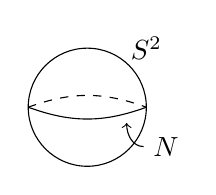
\begin{tikzpicture}
		\draw (0,0) circle (0.75); \draw[dashed] (-0.75,0) to[out=20,in=160] (0.75,0); \draw (-0.75,0) to[out=340,in=200] (0.75,0);
		\node at (0.75,0.75) {$S^2$}; \node (N) at (1,-0.5) {$N$};
		\draw[->] (N) to[out=180,in=270] (0.5,-0.2);
	\end{tikzpicture}\end{center}
	\begin{description}[font=\normalfont\itshape]
	\item[Behauptung:]
		$N$ ist eine Untermannigfaltigkeit von $M$.\marginnote{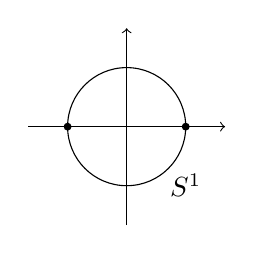
\begin{tikzpicture}
			\draw[->] (-1.25,0) -- (1.25,0); \draw[->] (0,-1.25) -- (0,1.25);
			\draw (0,0) circle (0.75); \fill (-0.75,0) circle (0.05) (0.75,0) circle (0.05); \node at (0.75,-0.75) {$S^1$};
		\end{tikzpicture}}
	\item[Beweis:]
		Sei $\varphi: \overbrace{S^n \setminus \{(1, 0,\ldots ,0)\}}^{=:U} \to \R^n$, $\varphi(x) = \frac{1}{1-x^0}(x^1,\ldots ,x^n)$
		
		\emph{Zu zeigen:} $\varphi(U \cap N) = \varphi(U) \cap (\R \times \{0\}^{n-1})$
			\[ \varphi(U \cap N) = \varphi(N \setminus \{(1,\ldots ,0)\}) = \R \times \{0\}^{n-1} \]
		F"ur $p \in N \setminus \{(1,0, \ldots ,0)\}$ ist $\varphi$ also eine adoptierte Karte um $p$. F"ur $p = (1, 0, \ldots, 0)$ ist analog $\psi$ (aus 1 a)) eine adoptierte Karte.
	\end{description}
\item
	$M = \R^2$, $N = \{(x, 0) | x \ge 0\} \cup \{(0,y)|y \ge 0\}$; Skizze:
	\begin{center}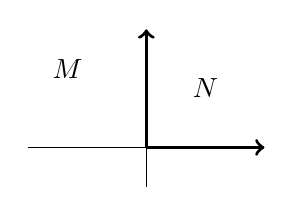
\begin{tikzpicture}
		\draw (-1.5,0) -- (0,0); \draw[very thick,->] (0,0) -- (1.5,0);
		\draw (0,-0.5) -- (0,0); \draw[very thick,->] (0,0) -- (0,1.5);
		\node at (-1,1) {$M$}; \node at (0.75,0.75) {$N$};
	\end{tikzpicture}\end{center}
	\begin{description}[font=\normalfont\itshape]
	\item[Behauptung:]
		$N$ ist keine glatte Untermannigfaltigkeit von $\R$.
	\item[Beweis:]
		Angenommen $N$ w"are Untermannigfaltigkeit von $\R^2$. Da $N$ hom"oomorph zu $\R$ ist, w"are es eine eindimensionale Untermannigfaltigkeit. Damit existiert eine Karte $(\varphi, U)$ von $\R^2$ um $(0,0)$ mit $\varphi(U\cap N) = \varphi(U) \cap (\R \times \{0\})$. Betrachte $\varphi^{-1}$, beziehungsweise $f(t) = \varphi^{-1}(t,0)$. Es sei $t_0 \in \R$ mit $f(t_0) = (0,0)$. Da $f(t) = N \cap U$ ist entweder $f(t) \in \{(0, y) | y \ge 0\}$ f"ur $t > t_0$ und $f(t) \in \{(x, 0) | x \ge 0\}$ f"ur $t < t_0$ oder umgekehrt. Dann ist $f'(t) \in \R e_2$ f"ur $ t > t_0$ und $f'(t) \in \R e_1$ f"ur $t < t_0$ oder umgekehrt.
		
		$\Rightarrow f'(0) \in \R e_1 \cap \R e_2 = \{(0,0)\}$
		
		\emph{Andererseits:} $f'(0) = \underbrace{(D \varphi^{-1}|_{\varphi(0,0)})}_{\text{Isom., da } \varphi^{-1} \text{ Diffeom.}}(\left(\begin{smallmatrix}1\\0\end{smallmatrix}\right)) \ne \left(\begin{smallmatrix}1\\0\end{smallmatrix}\right)$
	\end{description}
\end{enumerate}\end{Loes}